%  ALU_Design.tex
%  Document created by seblovett on seblovett-Ubuntu
%  Date created: Thu 17 Apr 2014 15:00:33 BST
%  <+Last Edited: Mon 12 May 2014 10:27:10 BST by seblovett on seblovett-Ubuntu +>


\section{Arithmetic Logic Unit}\label{sect:design:alu}
%\review{Arithmetic Logic Unit Design}
%\todo[color=cyan, inline]{Layout in silicon}

The ALU is the central unit for performing calculations within the datapath. 
Most instructions use the ALU as part of their operation and as such this module needs to interpret every instruction and perform the necessary function. 
The functions implemented fall into one of four types: arithmetic, logic, shifting and load lower. 
%With the last type being a special case for the LLI instruction. 
Arithmetic operations are centralised around a full adder.
Additional gates are used for subtraction and flag calculations. %setting the first input to zero and flag calculations. 
The logic operations consists of the gate corresponding to each of the logic instructions supported. 
Shifts are performed using a logarithmic shifter to support up to a 15 bit shift in one clock cycle. 
Finally, the LLI module concatenates the upper byte of the destination register with the provided 8 bit immediate value. 
The breakdown of the ALU is illustrated in Figure~\ref{fig:ALUModules}, with the output of each section connected to an internal bus through a number of tristate buffers. 

\todo[inline]{Redo Figures in \ref{ig:ALUAbsract} and \ref{fig:ArithLogicSlice}}
\begin{figure}[h]
	\centering
	\subfloat[Modular ALU Layout\label{fig:ALUModules}]{
	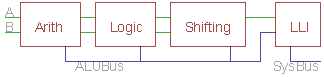
\includegraphics[width=3in]{Figures/AbstractALU.png}
	}
	\subfloat[Top-Level View of ALU\label{fig:BasicALUSym}]{
	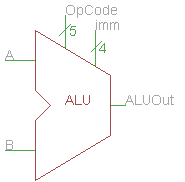
\includegraphics[width=1.6in]{Figures/ALUTopLevel.png}
	}
	\caption{ALU Abstraction}
	\label{fig:ALUAbsract}
\end{figure}

This design then needed to be bit sliced to simplify the datapath and promote hierarchical construction. 
It was decided to add an additional input to the module for the 4 bit immediate value required to define the shifting amount. 
Otherwise the lowest four slices of the ALU would each need different routing to each segment, reducing how much of each slice could be identically duplicated. 

Initial design of the ALU module was based upon the planned datapath layout as shown in Figure~\ref{fig:BasicALUSym}. 
From this it was seen that there may be some difficulty with interpreting the Opcodes provided. 
Each slice would have to individually interpret the Opcode, using much more space than is necessary due to replicated hardware. 
Observations showed that different groups of instructions would perform the same operation within the ALU, therefore a separate decoder module was implemented to reduce required area.

\subsection{ALU Slice}
%The arithmetic section was simple to bitslice since the full adder and input selection gates would be duplicated for each bit anyway. 
%While the flags required only one OR gate for the Z flag and the sum, carry in and carry out signals to be available at the top of the slice. 
%Since a decoder is positioned at the top, additional gates needed for flag calculation can be implemented once within the decoder. 
%This is shown in Figure~\ref{fig:ArithSlice}. 
%Bit slicing the logic section was just one of each logic gate followed by a tri-state buffer in the slice, shown in Figure~\ref{fig:LogicSlice}. 
Due to the regularity of the ALU, the bit slice was simple to implement.
The zero flag was calculated using an OR gate in each slice, which is then inverted in the decoder.
Carry and negative flags are available using the outputs of the top slice. 
The overflow flag is calculated using the top slice outputs in the decoder.
The arithmetic implementation is shown in Figure~\ref{fig:ArithSlice}. 
The logic operations were simple to implement, using the logic gates, each with a tristate buffer to the output bus.
The circuit diagram is shown in Figure~\ref{fig:LogicSlice}.


\begin{figure}[h]
	\centering
	\subfloat[Arithmetic Section\label{fig:ArithSlice}]{
	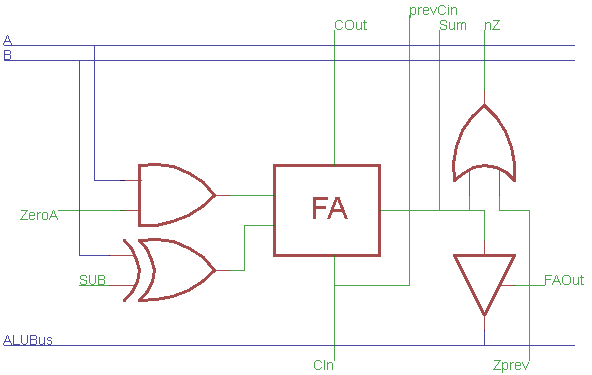
\includegraphics[scale=0.75]{Figures/ArithSlice.png}
	}
	\subfloat[Logic Section\label{fig:LogicSlice}]{
	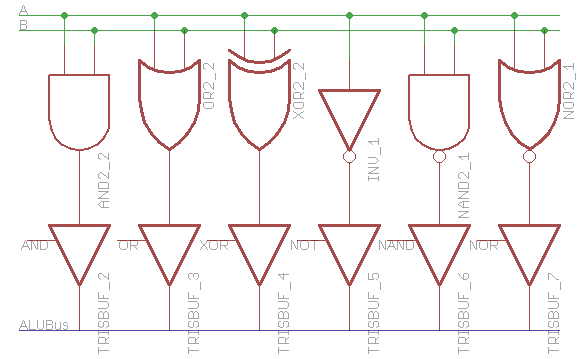
\includegraphics[scale=0.75]{Figures/LogicSlice.png}
	}
	\caption{Bitsliced Circuit Diagrams for Arithmetic and Logic Sections}
	\label{fig:ArithLogicSlice}
\end{figure}

%\begin{figure}[h]
%	\centering
%	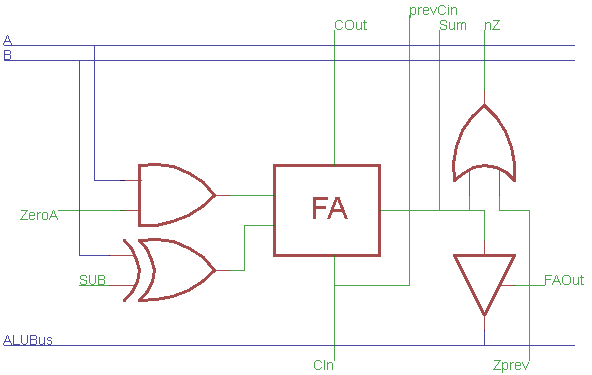
\includegraphics[scale=0.75]{Figures/ArithSlice.png}
%	\caption{Bitsliced Ciruit Diagram for Arithmetic Section of ALU}
%	\label{fig:ArithSlice}
%\end{figure}

%\begin{figure}[h]
%	\centering
%	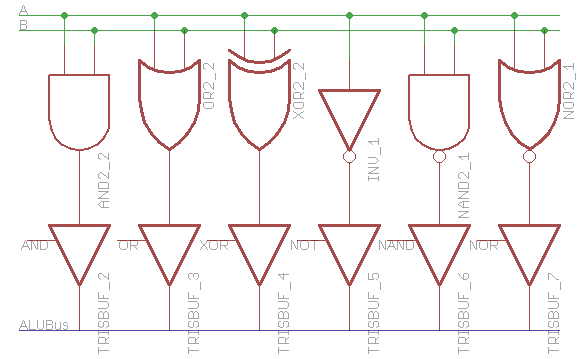
\includegraphics[scale=0.75]{Figures/LogicSlice.png}
%	\caption{Bitsliced Ciruit Diagram for Logic Section of ALU}
%	\label{fig:LogicSlice}
%\end{figure}

Implementing shifting capabilities into individual bits required few logic gates since it is a wire-dominated circuit, but each wire needed to be lined up correctly between slices. 
This results from this slice section having more dependency on the neighbouring slices than both arithmetic and logic functions. 
The left and right shifting have been implemented using separate hardware, with a logarithmic strategy. 
To support arithmetic shifting, the shifted value into a right shift can be either a zero or the current operand's sign.
Implementation of this section is shown in Figure~\ref{fig:ShiftSlice}. 


\begin{figure}[h]
	\centering
	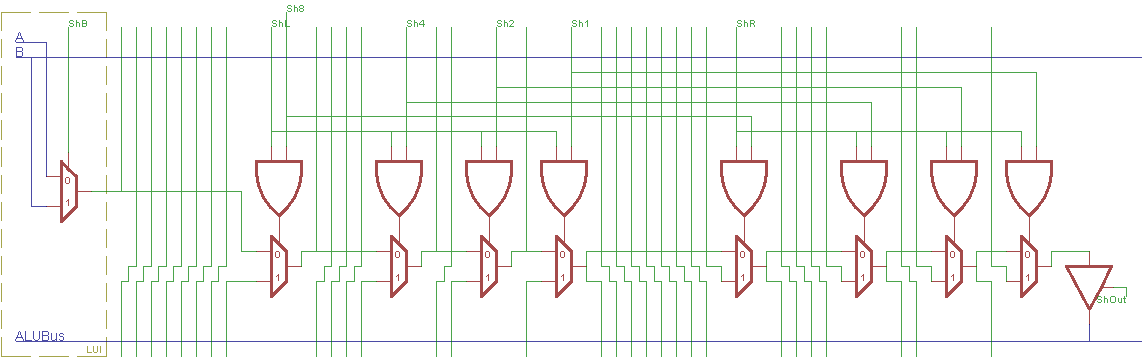
\includegraphics[width=\textwidth]{Figures/ShiftSlice.png}
	\caption{Bitsliced Circuit Diagram for Shift Section of ALU}
	\label{fig:ShiftSlice}
\end{figure}

Every instruction can be carried out using one of the previous sections, with the exception of \textbf{LUI} and \textbf{LLI}. 
Loading an upper immediate value involves concatenating the 8 bit value with 8 zero bits. 
This is equivalent to shifting the second operand by 8 bits, as such it can be implemented with an additional multiplexor before the shifting section to select between each input operand. 
This is shown in Figure~\ref{fig:ShiftSlice} as a precursor to standard shifting operation. 
Loading a lower immediate involves concatenating the existing high byte of the destination register with the value in the instruction. 
However, it is not possible to separate this into 16 identical slices. 
As such two versions of the slice were designed, one which passes through the upper byte with no change, and one which selects between the lower byte of the input register value and the immediate value. 
These form modules which are separate to the main slice consisting of either wiring or a multiplexor.

\subsection{ALU Decoder}
The purpose of a decoder module is to convert any given Opcode into a number of signals to control the path of data within the ALU. 
As such it is composed of combinational logic. 
Table~\ref{tab:contrOuts} shows the necessary control signals for each mnemonic.

\begin{table}[h]
	\caption{Control outputs for each available instruction mnemonic}
	\label{tab:contrOuts}
	\centering
	\footnotesize
	\makebox[\linewidth]{
	\begin{tabular}{|r|l|l|c|r|l|l|}
		\multicolumn{2}{c}{Instruction} & \multicolumn{1}{c}{Decoder Outputs} & \multicolumn{1}{c}{\hspace{0.5cm}} & \multicolumn{2}{c}{Instruction} & \multicolumn{1}{c}{Decoder Outputs} \\
		\cline{1-3} \cline{5-7} 
		LDW   & 00000 & FAOut &  & NOP   & 11000 & ShOut \\
		POP   & 00001 & FAOut &  & 'F'   & 11001 & ShOut \\
		ADDIB & 00011 & FAOut &  & NEG   & 11010 & FAOut, SUB, ZeroA \\
		ADD   & 00010 & FAOut &  & 'D'   & 11110 & FAOut \\
		ADDI  & 00110 & FAOut &  & LSL   & 11111 & ShOut, ShL, \{Sh8-1\} \\
		CMP   & 00111 & FAOut, SUB &  & LSR   & 11101 & ShOut, ShR, \{Sh8-1\} \\
		ADCI  & 00101 & FAOut, {\it UseC} &  & ASR   & 11100 & ShOut, ShR, {\it ShSign}, \{Sh8-1\} \\
		ADC   & 00100 & FAOut, {\it UseC} &  & AND   & 10000 & AND \\
		STW   & 01000 & FAOut &  & OR    & 10001 & OR \\
		PUSH  & 01001 & FAOut, SUB &  & XOR   & 10011 & XOR \\
		SUBIB & 01011 & FAOut, SUB &  & NOT   & 10010 & NOT \\
		SUB   & 01010 & FAOut, SUB &  & NAND  & 10110 & NAND \\
		SUBI  & 01110 & FAOut, SUB &  & NOR   & 10111 & NOR \\
		CMPI  & 01111 & FAOut, SUB &  & LLI   & 10101 & ShOut, LLI \\
		SUCI  & 01101 & FAOut, SUB, {\it UseC} &  & LUI   & 10100 & ShOut, ShL, ShB, Sh8 \\
		SUC   & 01100 & FAOut, SUB, {\it UseC} &  & & 11011 & - \\
		\cline{1-3} \cline{5-7}
	\end{tabular}
	}

\end{table}

\textit{SUB} inverts the second input and flags for a subtraction operation and \textit{ZeroA} sets the first input to zero. 
\textit{ShL} and \textit{ShR} switch between left and right shifting while \textit{ShB} switches between using the first (A) or second (B) input to shift. 
Signals \textit{Sh8}, \textit{Sh4}, \textit{Sh2} and \textit{Sh1} enable each section of the barrel shifter and during normal shifting operations are dependent upon the 4 bit immediate input to decoder. 
\textit{Sh8} is set during a \textbf{LUI} instruction since it will always shift by 8 bits. 
Signal \textit{LLI} activates the LLI module after no operation is performed within the main ALU. 
While \textit{UseC} and \textit{ShInBit} are internal signals indicating use of the carry flag from previous instruction and the bit to shift in respectively. 
The remaining signals enable the relevant tristate buffers to output the result. It uses one hot encoding to prevent contention. 
The one unused Opcode does not activate any signals to reduce the number of gates within the decoder. 

\begin{align}
	\text{FAOut} &= \bar{A} + BD\bar{E} \label{eq:DecBasicS}\\
	\text{SUB} &= \bar{A}BC + \bar{A}B\bar{C}E + B\bar{C}D\bar{E} + \bar{A}CDE \\
	\text{ShL} &= ABCDE + A\bar{B}C\bar{D}\bar{E} \\
	\text{Sh8} &= (ABCE + ABC\bar{D})imm[3] + A\bar{B}C\bar{D}\bar{E} \\
	\text{Sh4} &= (ABCE + ABC\bar{D})imm[2] \\
	\text{Sh2} &= (ABCE + ABC\bar{D})imm[1] \\
	\text{Sh1} &= (ABCE + ABC\bar{D})imm[0] \\
	\text{ShOut} &= AC\bar{D} + ABCE + AB\bar{C}\bar{D} \\
	\text{UseC} &= \bar{A}C\bar{D} \\
	\text{ShR} &= ABC\bar{D} \label{eq:DecBasicF}
\end{align}

By using the Opcodes and K-map groupings defined in Table~\ref{tab:OpKmaps}, logic equations have been formed as shown in Equations~\eqref{eq:DecBasicS}~to~\eqref{eq:DecBasicF}. 
Where the letters A-E correspond to bits 4-0 of the Opcode. 
Refining these equations for implementation considered the set of logic gates available within the library, as well as the number of gates needed. 
Since the negated output gates could have more inputs, as well as being physically smaller, they were more favourable to use. 
Some potential options for the logic equation for the \textit{SUB} signal are shown in Equations~\eqref{eq:DecSUB1}~and~\eqref{eq:DecSUB2}. 
The first one, taken from the K-map, requires 9 non-inverting logic gates. 
%To simplify design, inverters were not considered for optimization as both inverted and non-inverted inputs were made available globally. 
This equation cannot be implemented since \texttt{AND} gates with more than 2 inputs are not available. 
Equation~\eqref{eq:DecSUB2} requires 8 gates and cannot be implemented using the available library.
However if inverted using DeMorgan's law to produce Equation~\eqref{eq:DecSUB3} it is possible.
Since no further improvements could be made, this final equation is used and implemented in Figure~\ref{fig:DecMultiCirs}. A similar approach was used for the remaining signals, also shown in Figure~\ref{fig:DecMultiCirs}. 

The additional logic needed for the flag calculations is implemented in the decoder. 
However, the circuit diagram for this portion is shown in Figure~\ref{fig:DecMultiCirs}. 
For the control signals which respond to only one Opcode, a gate array was used, as shown in Figure~\ref{fig:GateArray}. 

\newcommand{\overbar}[1]{\mkern 1.5mu\overline{\mkern-1.5mu#1\mkern-1.5mu}\mkern 1.5mu}
\begin{align}
	\text{SUB} &= \bar{A}BC + \bar{A}B\bar{C}E + B\bar{C}D\bar{E} + \bar{A}CDE \label{eq:DecSUB1}\\
	&= \bar{A}B(C + \bar{C}E) + D(B\bar{C}\bar{E} + \bar{A}CE) \label{eq:DecSUB2}\\
	&= \overbar{\overbar{(\bar{A}B\overbar{(\bar{C}\overbar{(\bar{C}E)})})}\overbar{(D\overbar{(\overbar{(B\bar{C}\bar{E})}\overbar{(\bar{A}CE)})})}} \label{eq:DecSUB3}
\end{align}

\begin{figure}[h!]
	\centering
	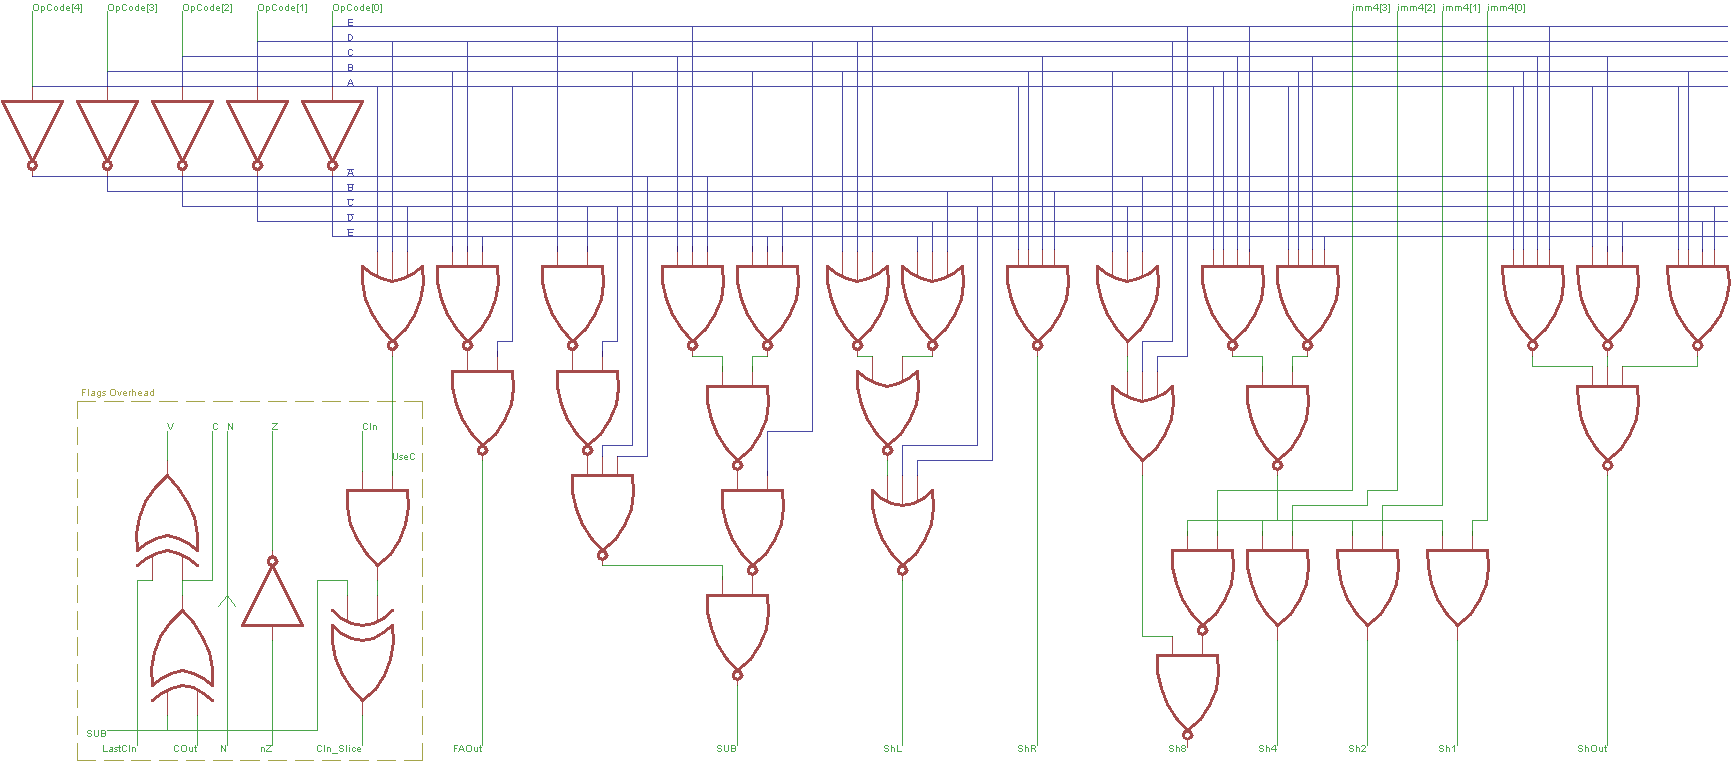
\includegraphics[width=\textwidth]{Figures/ALUDecoderMore1v2.png}
	\caption{Circuit Diagrams For Signals Active For More Than One Opcode}
	\label{fig:DecMultiCirs}
\end{figure}


\begin{figure}[h]
	\centering
	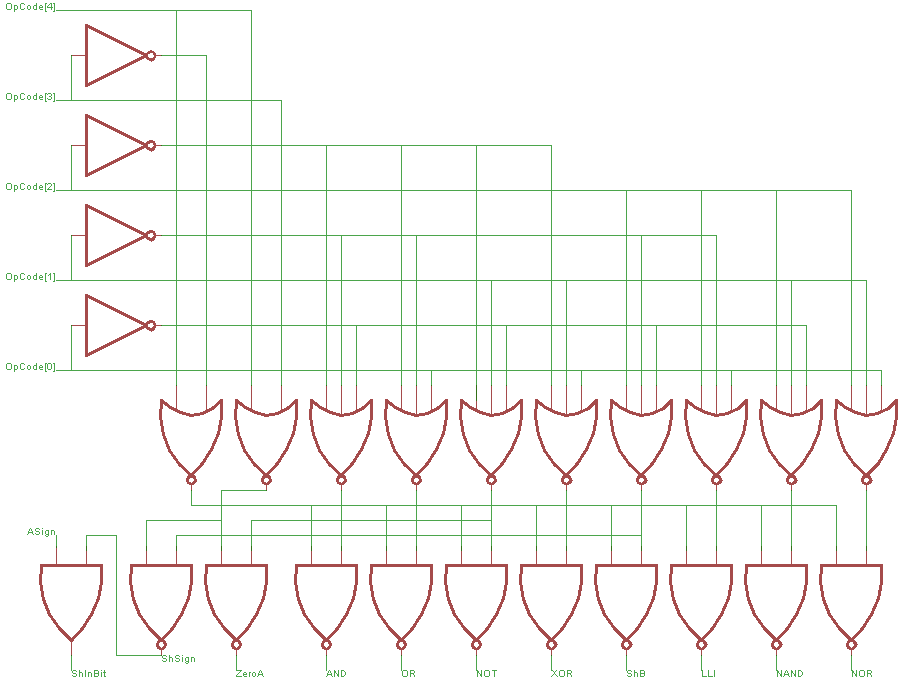
\includegraphics[scale=0.75]{Figures/ALUDecoderGateArrayv2.png}
	\caption{Circuit Diagrams For Gate Array and Flag Overhead Logic}
	\label{fig:GateArray}
\end{figure}

\subsection{ALU Block}
The final hierarchical view of the assembled ALU made up of each part mentioned previously is shown in Figure~\ref{fig:ALUAssembled}. 
ALU slice is duplicated to make up the 16 bits in parallel, LLI high is added to the top half and LLI low is added to the bottom half. 
The decoder is added above, with additional wiring to connect together right shifting inputs. 
The left shifting inputs at the bottom are tied to ground. 
The output to the ALU is available as a direct connection to the rest of the datapath, but it is also stored in a register for later transfer onto the system bus. 
This register forms a part of a separate module to the ALU. 

\begin{figure}[h]
	\centering
	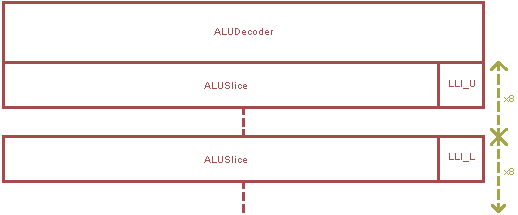
\includegraphics[scale=0.75]{Figures/ALUModular.png}
	\caption{Modular Diagram of Assembled ALU}
	\label{fig:ALUAssembled}
\end{figure}
